\section{Results}   \label{sec:results}
% Results



%% Able to approximate the feasable control region by solving QP over large displacement space
Using our model-based control approach we have been able to control the position of the end effector of a linear/rotary 2DOF system with a root-mean-square error of less than --- m in linear displacement and --- $^\circ$ in rotation over a set of --- test points. This amounts to a control accuracy of within --- \% of the acheivable range of linear displacements, and --- \% of the achievable range of rotations.

%% Description of system
These preliminary results were achieved on a system comprised of a parallel configuration of three FREE actuators constrained to only linear and rotary displacements (Figure \ref{fig:modules}), as described in section \ref{sec:experiments}. All three actuators had a nominal radius and length of 5 mm and 100 mm, respectively. In order to ensure that both clockwise and counterclockwise rotations would be attainable, a counterclockwise twisting FREE with reinforcing fiber wrapped at a ---$^\circ$ angle with respect to horizontal, and a clockwise twisting FREE with the fiber wrapped at a ---$^\circ$ angle were both used, as well as another ----- twisting FREE with fiber wrapped at a ---$^\circ$ angle. Each of these FREEs is also of the contracting type, which is why the workspace lies entirely to the left of the origin in figure \ref{fig:results}.


%% Plot comparing the the desired end effector positions to those achieved
\begin{figure}
    \centering
    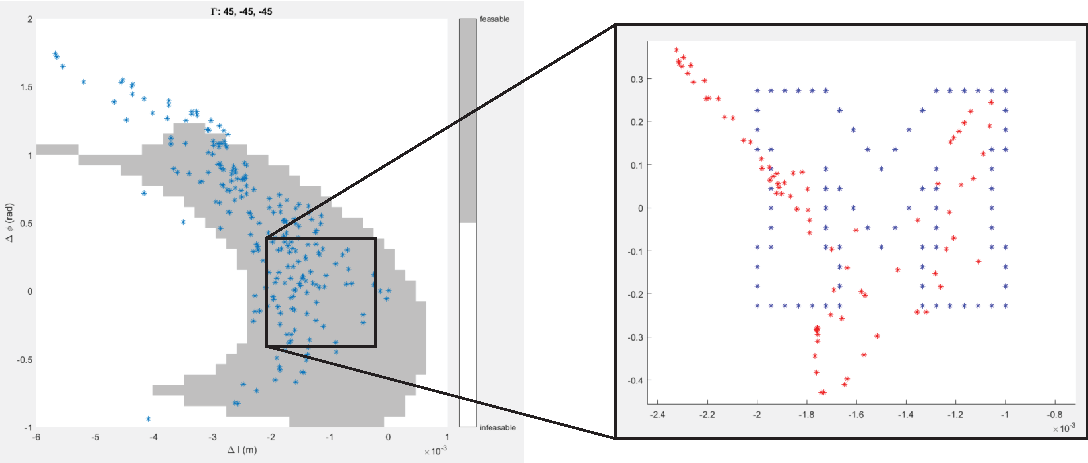
\includegraphics[width=\linewidth]{figures/resultsDiagram.pdf}
    \caption{(a) The feasable control region calculated by the model with measured test points over range of admissable pressures superimposed. (b) Desired end effector positions compared to measured end effector positions at corresponding pressures. \Dan{Placeholder figure and caption just to show the proposed structure. Didn't want to waste time nicely formatting bad results.}}
    \label{fig:results}
\end{figure}

